\documentclass[a4paper,11pt]{report}
\usepackage[slovene]{babel}
\usepackage{listings}
\usepackage{graphicx}
\usepackage[section]{placeins}

\lstset{
numberstyle=\small, 
numbersep=8pt, 
frame = single, 
language=SQL, 
framexleftmargin=15pt}

\begin{document}

\title{TUP: 4. domača naloga}
\author{Jakob Marušič}
\maketitle

\section*{Naloga (a)}

\paragraph{Navodila}
\begin{em}
    Prvi del naloge se navezuje na vašo dosedanjo serijo domačih nalog. Za vašo  opišite vsaj eno smiselno aktivnost z več opravili (npr. zapis rezultatov preiskav) in jo realizirajte v obliki ene ali več transakcij. Vašo rešitev ustrezno dokumentirajte.
\end{em}

\paragraph{Opis opravila} Pacient je bil udeležen v prometni nesreči in je lažje poškodovan bil pripeljan v zdravstveni dom z
vozilom nujne medincinske pomoči. Zdravstveno osebje ga mora zapisati v register pacientov ter za njega odpreti novo obravnavo in ga uvrstiti na čakalno vrsto.
\\\\\textit{Spodnja SQL koda se navezuje na podatkovno bazo iz druge domače naloge.}

\paragraph{}\mbox{}
\begin{lstlisting}[language=SQL]
SET autocommit = OFF

START TRANSACTION;
    
    INSERT IGNORE INTO kraj 
        (postna_stevilka, kraj) 
        VALUES (1000, 'Ljubljana')

    INSERT IGNORE INTO naslov 
        (ulica, hisna\_stevilka, postna\_stevilka) 
        VALUES ('Vecna pot', 113, 1000)
    
    INSERT IGNORE INTO pacient 
        (stevilka_kzz, ime, priimek, 
            rojstni_datum, spol) 
        VALUES (50021, 'Pinko', 'Palinko', 
            1970-01-01, 'M')
    
    INSERT INTO obravnava 
        (stevilka_kzz) 
        VALUES (50021)

    INSERT INTO cakalna_vrsta 
        (datum_vpisa, cas_vpisa, stevilka_oddelka) 
        VALUES (CURRENT_DATE(), CURRENT_TIME(), 5023)

COMMIT;
\end{lstlisting}


\section*{Naloga (b)}
\paragraph{Navodila}
\begin{em}
    Drugi del sloni na nalogah, ki smo jih opravljali na vajah v okviru sočasnega dostopa do PB. Z uporabo večnitnega programiranja v Pythonu simulirajte množico sočasnih dostopov do podatkov. 
    \\Z uporabo podprogramov iz vaj (po potrebi s popravki) nad podatki iz prejšnjih domačih nalog reproducirajte štiri težave sočasnega dostopa:
    \begin{enumerate}
        \item branje nepotrjenega podatka (dirty read)
        \item neponovljivo branje oz. nekonsistentna analiza (non-repeatable read)
        \item branje fantomskega podatka (phantom read)
        \item izgubljeno ažuriranje
    \end{enumerate}

    Nato rešite težave z uporabo transakcijskih ukazov in stopnje izolacije transakcij.
\end{em}

\pagebreak
\subsection*{Branje nepotrjenega podatka (dirty read)}

\paragraph{Python skripta}\mbox{}

\begin{lstlisting}[showstringspaces=false][language = Python]
def vstavi():
    db = connect()
    cursor = db.cursor()
    x = 100100
    for i in range(1):
        query = "INSERT INTO ODDELEK(sifra_oddelka)\
         VALUES (%s)"
        cursor.execute(query, [x])
        x += 1
        time.sleep(10)

def beriOddelek():
    db = connect()
    cursor = db.cursor()
    time.sleep(0.25)
    cursor.execute("SELECT * FROM ODDELEK")
    rez = cursor.fetchall()
    for row in rez:
        print(row[0])

    
def dirtyRead():
    db = connect()
    cursor = db.cursor()
    cursor.execute("SET GLOBAL TRANSACTION ISOLATION 
    LEVEL READ UNCOMMITTED")
    Thread(target = vstavi).start()
    Thread(target = beriOddelek).start()
    time.sleep(10)
    Thread(target = beriOddelek).start()

dirtyRead()
\end{lstlisting}

\paragraph{Komentar rešitve}
Branje nepotrjenega podatka se pripeti, ko prva transakcija (naš primer \textit{vstavi()}) vstavlja/spreminja
podatek, ki ga druga transakcija (\textit{beriOddelek()}) bere preden ga prva dejansko potrdi v bazi.\\\\
V kolikor prva transakcija podatka ne potrdi, se le ta ne zapiše v bazo, druga transakcija pa pri ponovitvi branja podatka ne prebere več (ker ga v bazi ni).

\paragraph{Tabelaričen povzetek eksperimenta}\mbox{}

\noindent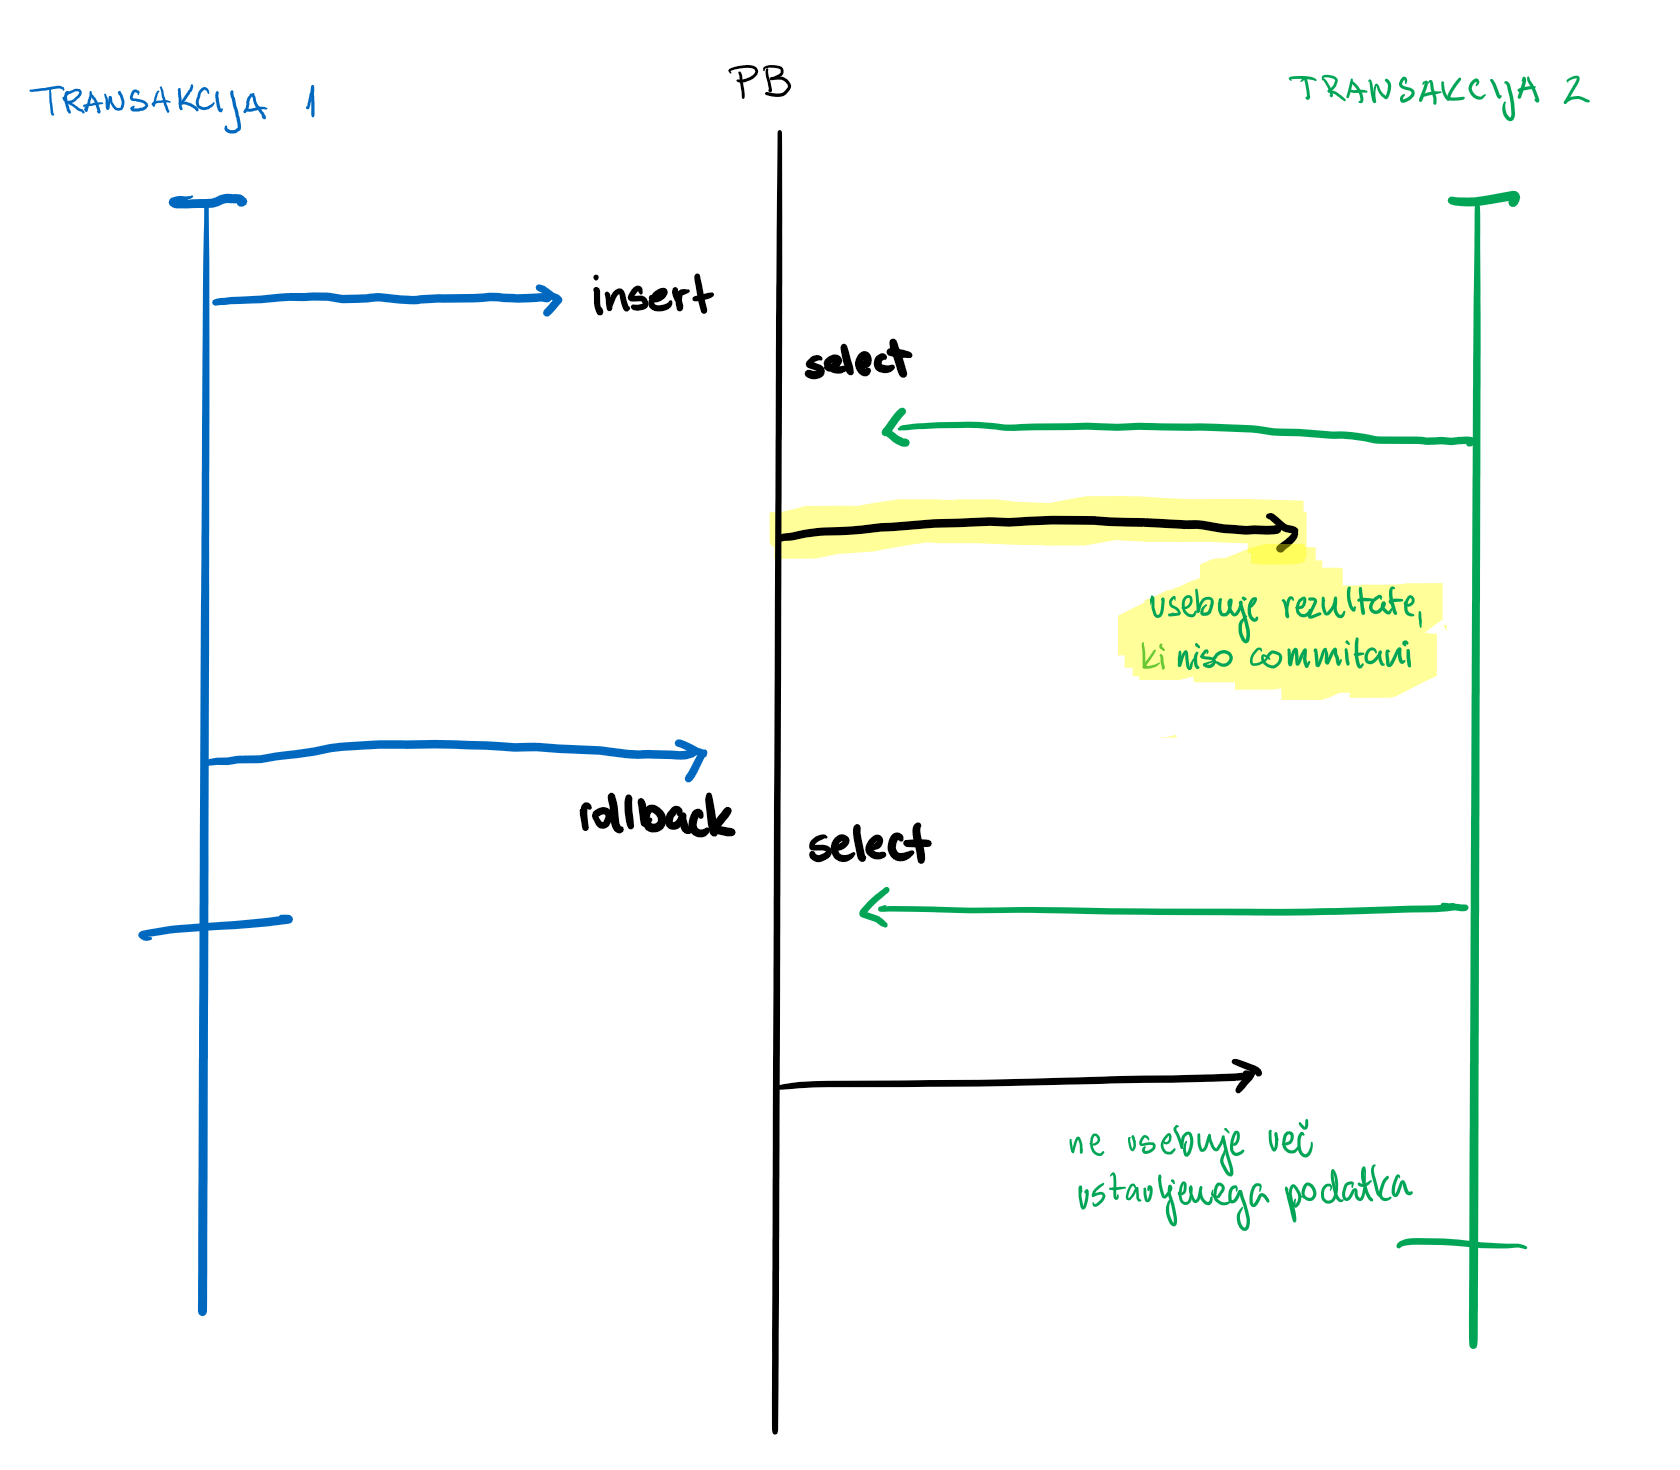
\includegraphics[width=\linewidth]{./pics/dirty-read.png}

\paragraph{Rešitev}
Branje nepotrjenega podatka lahko preprečimo z uporabo stopnje izolacije \textit{READ COMMITTED}, \textit{REPEATABLE READ} in \textit{SERIALIZABLE}.

\pagebreak
\subsection*{Neponovljivo branje oz. nekonsistentna analiza (non-repeatable read)}

\paragraph{Python skripta}\mbox{}

\begin{lstlisting}[showstringspaces=false][language = Python]
def posodobiNonRepeatable():
    db = connect()
    cursor = db.cursor()
    time.sleep(2)
    query = "UPDATE pacient SET starost = 26\
        WHERE kzz = 500004"
    cursor.execute(query)
    db.commit()

def berinonRepeatable():
    db = connect()
    cursor = db.cursor()
    cursor.execute("SELECT * FROM PACIENT\
    WHERE kzz = 500004")
    rez = cursor.fetchone()
    print(rez)
    time.sleep(3)
    cursor.execute("SELECT * FROM PACIENT\ 
    WHERE kzz = 500004")
    rez = cursor.fetchone()
    print(rez)

def nonRepeatable():
    Thread(target = berinonRepeatable).start()
    Thread(target = posodobiNonRepeatable).start()

nonRepeatable()
\end{lstlisting}

\paragraph{Komentar rešitve}
Neponovljivo branje se zgodi, ko prva transakcija dvakrat bere podatek iz podatkovne baze, pri čemer se
podatek druga transakcija posodobi med obema branjema prve.

V primeru izolacijske stopnje \textit{READ COMMITTED} ali \textit{READ UNCOMMITTED} se pri drugem branju pojavi posodobljena verzija
podatka. Ta pojav imenujemo neponovljivo branje.
\pagebreak
\paragraph{Tabelaričen povzetek eksperimenta}\mbox{}

\noindent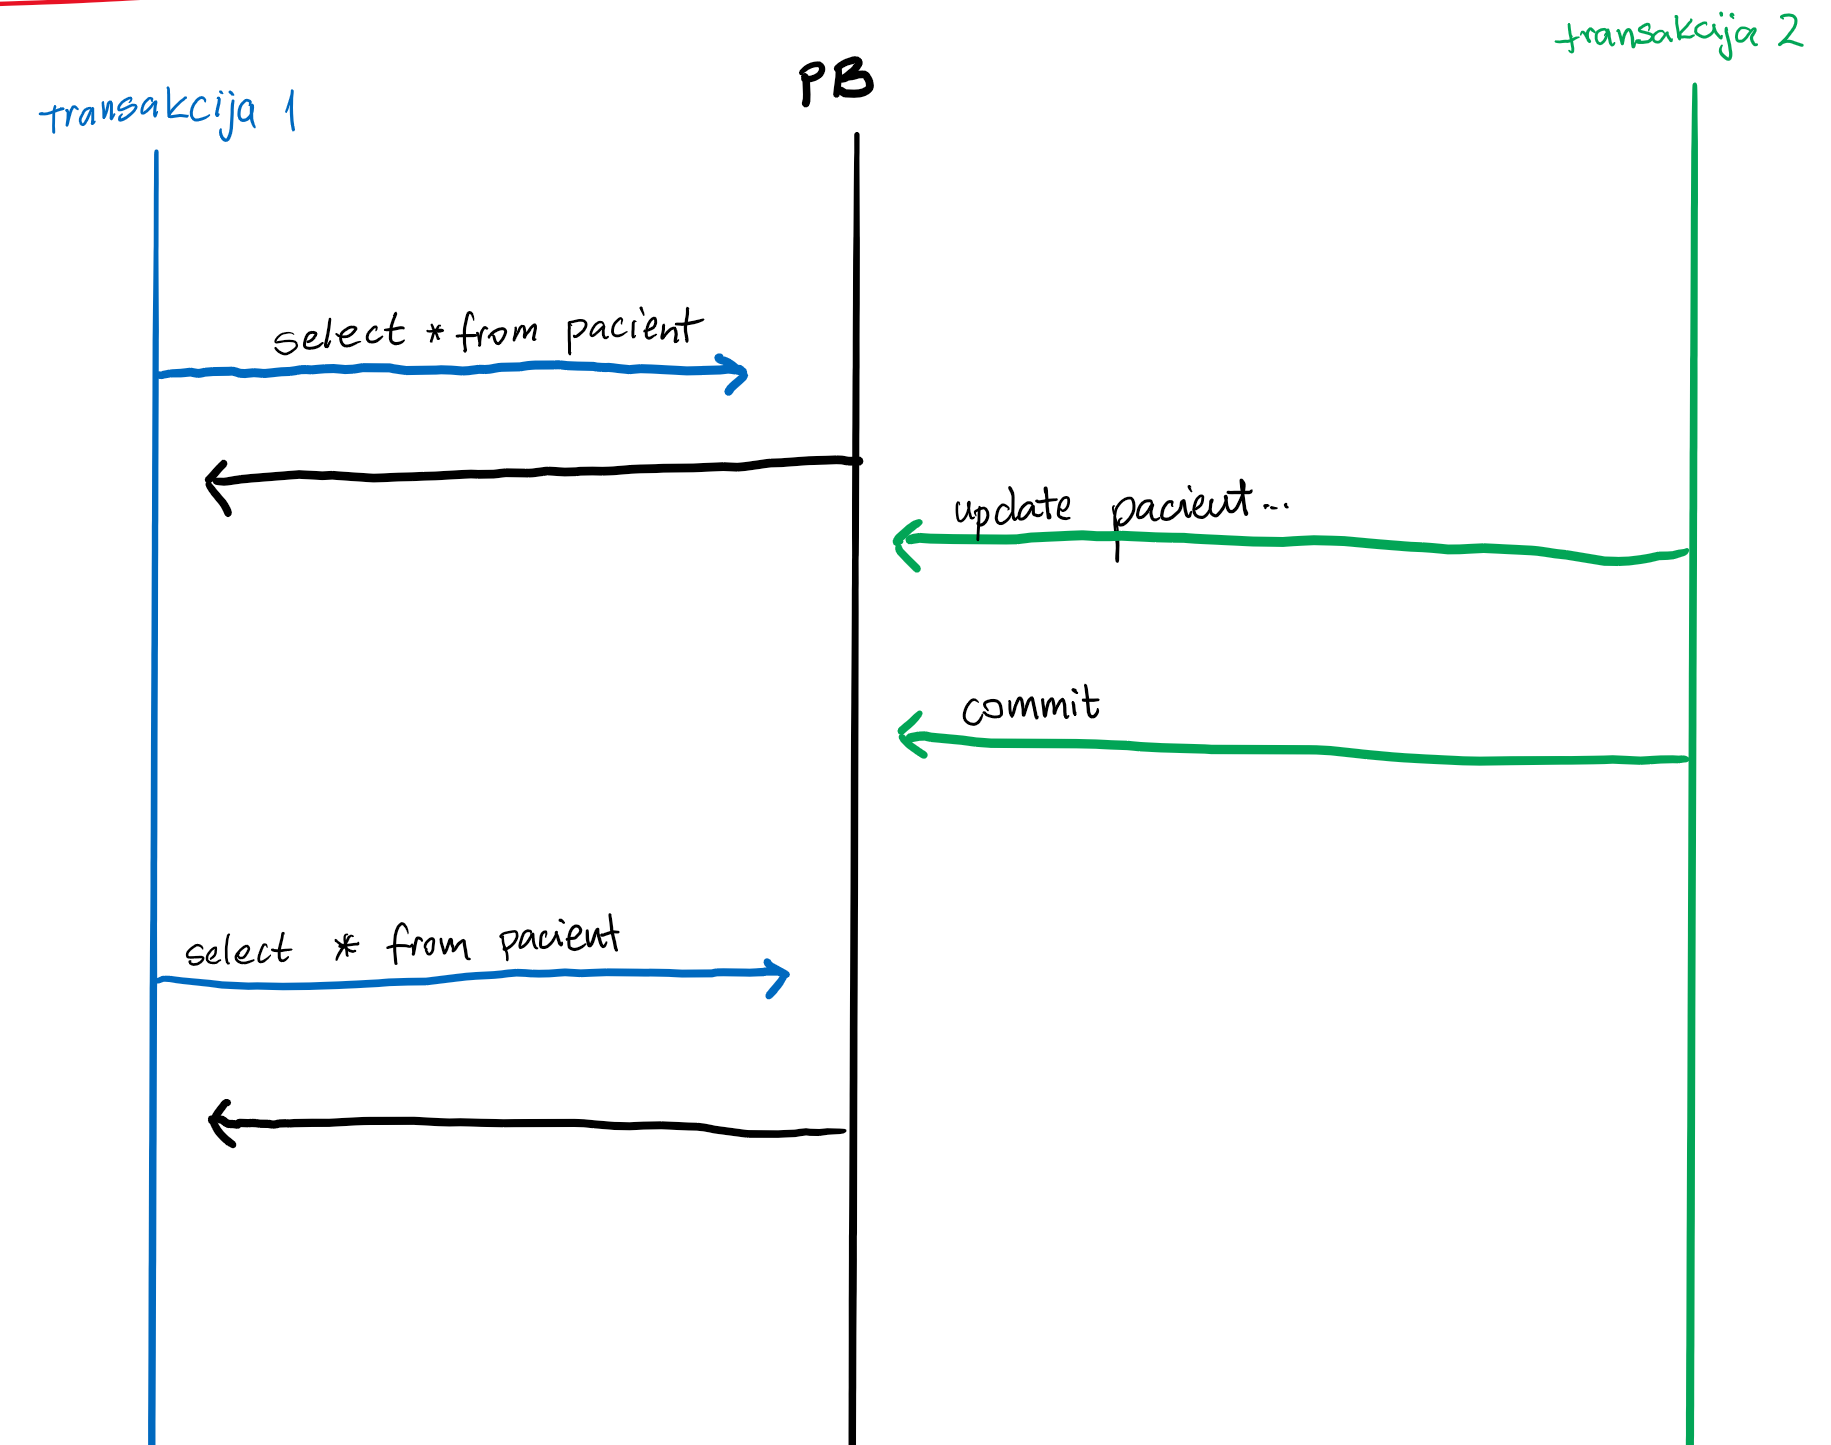
\includegraphics[width=\linewidth]{./pics/nonrepeatable.png}

\paragraph{Rešitev}
Neponovljivo branje lahko preprečimo z uporabo stopnje izolacije \textit{REPEATABLE READ} in \textit{SERIALIZABLE}.


\pagebreak
\subsection*{Branje fantomskega podatka (phantom read)}

\paragraph{Python skripta}\mbox{}
\begin{lstlisting}[showstringspaces=false][language = Python]
def vstaviPhantom():
    db = connect()
    cursor = db.cursor()
    time.sleep(2)
    query = "INSERT INTO\ 
        pacient(kzz, starost, spol)\ 
        VALUES (1110, 10, 'M')"
    cursor.execute(query)
    db.commit()

def beriPhanton():
    db = connect()
    cursor = db.cursor()
    cursor.execute("SELECT * FROM pacient\ 
        WHERE starost BETWEEN 10 AND 30\ 
        ORDER BY starost")
    rez = cursor.fetchall()
    for row in rez:
        print(row)
    time.sleep(3)
    cursor.execute("SELECT * FROM pacient\ 
        WHERE starost BETWEEN 10 AND 30\ 
        ORDER BY starost")
    rez = cursor.fetchall()
    for row in rez:
        print(row)

def phantonRead():
    Thread(target = beriPhanton).start()
    Thread(target = vstaviPhantom).start()

phantomRead()
\end{lstlisting}

\paragraph{Komentar}
Branje fantomskega podatka se zgodi, ko prva transakcija dvakrat bere enak set podatkov, vendar jih med obema branjema
neka druga transakcija spremeni (spremeni lahko en podatek ali več).

Gre za posebno obliko \textit{neponovljivega branja}.
\pagebreak
\paragraph{Tabelaričen povzetek eksperimenta}\mbox{}

\noindent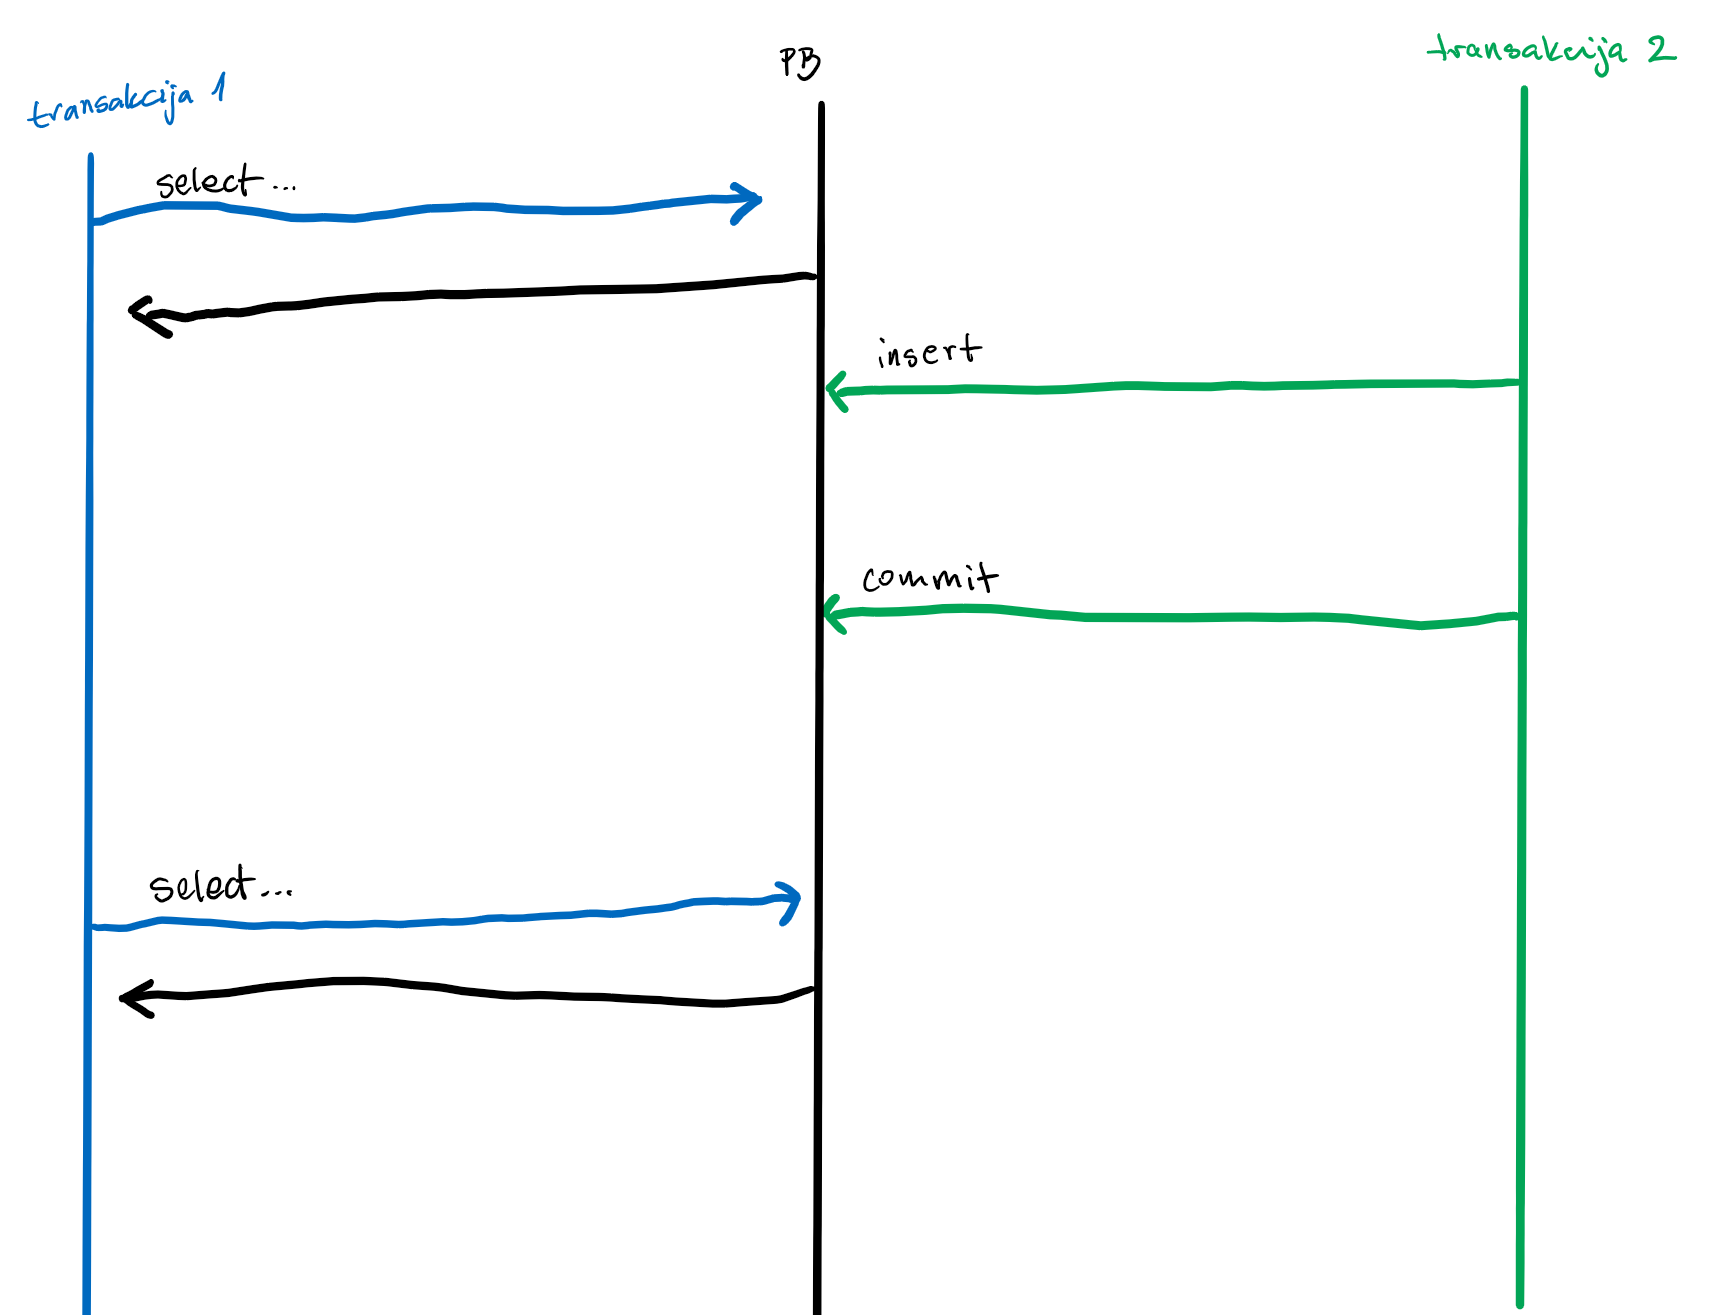
\includegraphics[width=\linewidth]{./pics/phantom.png}

\paragraph{Rešitev}
Fantomsko branje podatka lahko preprečimo z uporabo stopnje izolacije \textit{SERIALIZABLE}.


\pagebreak
\subsection*{Izgubljeno ažuriranje}
\paragraph{Python skripta}\mbox{}
\begin{lstlisting}[showstringspaces=false][language = Python]
def posodobi1():
    db = connect()
    cursor = db.cursor()
    query = "UPDATE pacient\ 
        SET starost = 96 WHERE kzz = 500004"
    cursor.execute(query)
    db.commit()

def posodobi2():o
    db = connect()
    cursor = db.cursor()
    query = "UPDATE pacient\ 
        SET starost = 97 WHERE kzz = 500004"
    cursor.execute(query)
    db.commit()

def beriAzuiranje():
    db = connect()
    cursor = db.cursor()
    cursor.execute("SELECT * FROM PACIENT\ 
        WHERE kzz = 500004")
    rez = cursor.fetchone()
    print(rez)

def azuriranje():
    Thread(target = posodobi1).start()
    Thread(target = posodobi2).start()
    time.sleep(2)
    Thread(target = beriAzuiranje).start()

azuriranje()

\end{lstlisting}


\paragraph{Komentar rešitve}
Izgubljeno ažuriranje se zgodi, ko dve transakciji (skoraj) istočasno posodabljata isti zapis v tabeli. V tabeli se ohrani samo zapis, ki je bil v tabelo zapisan kasneje.
\pagebreak
\paragraph{Tabelaričen povzetek eksperimenta}\mbox{}

\noindent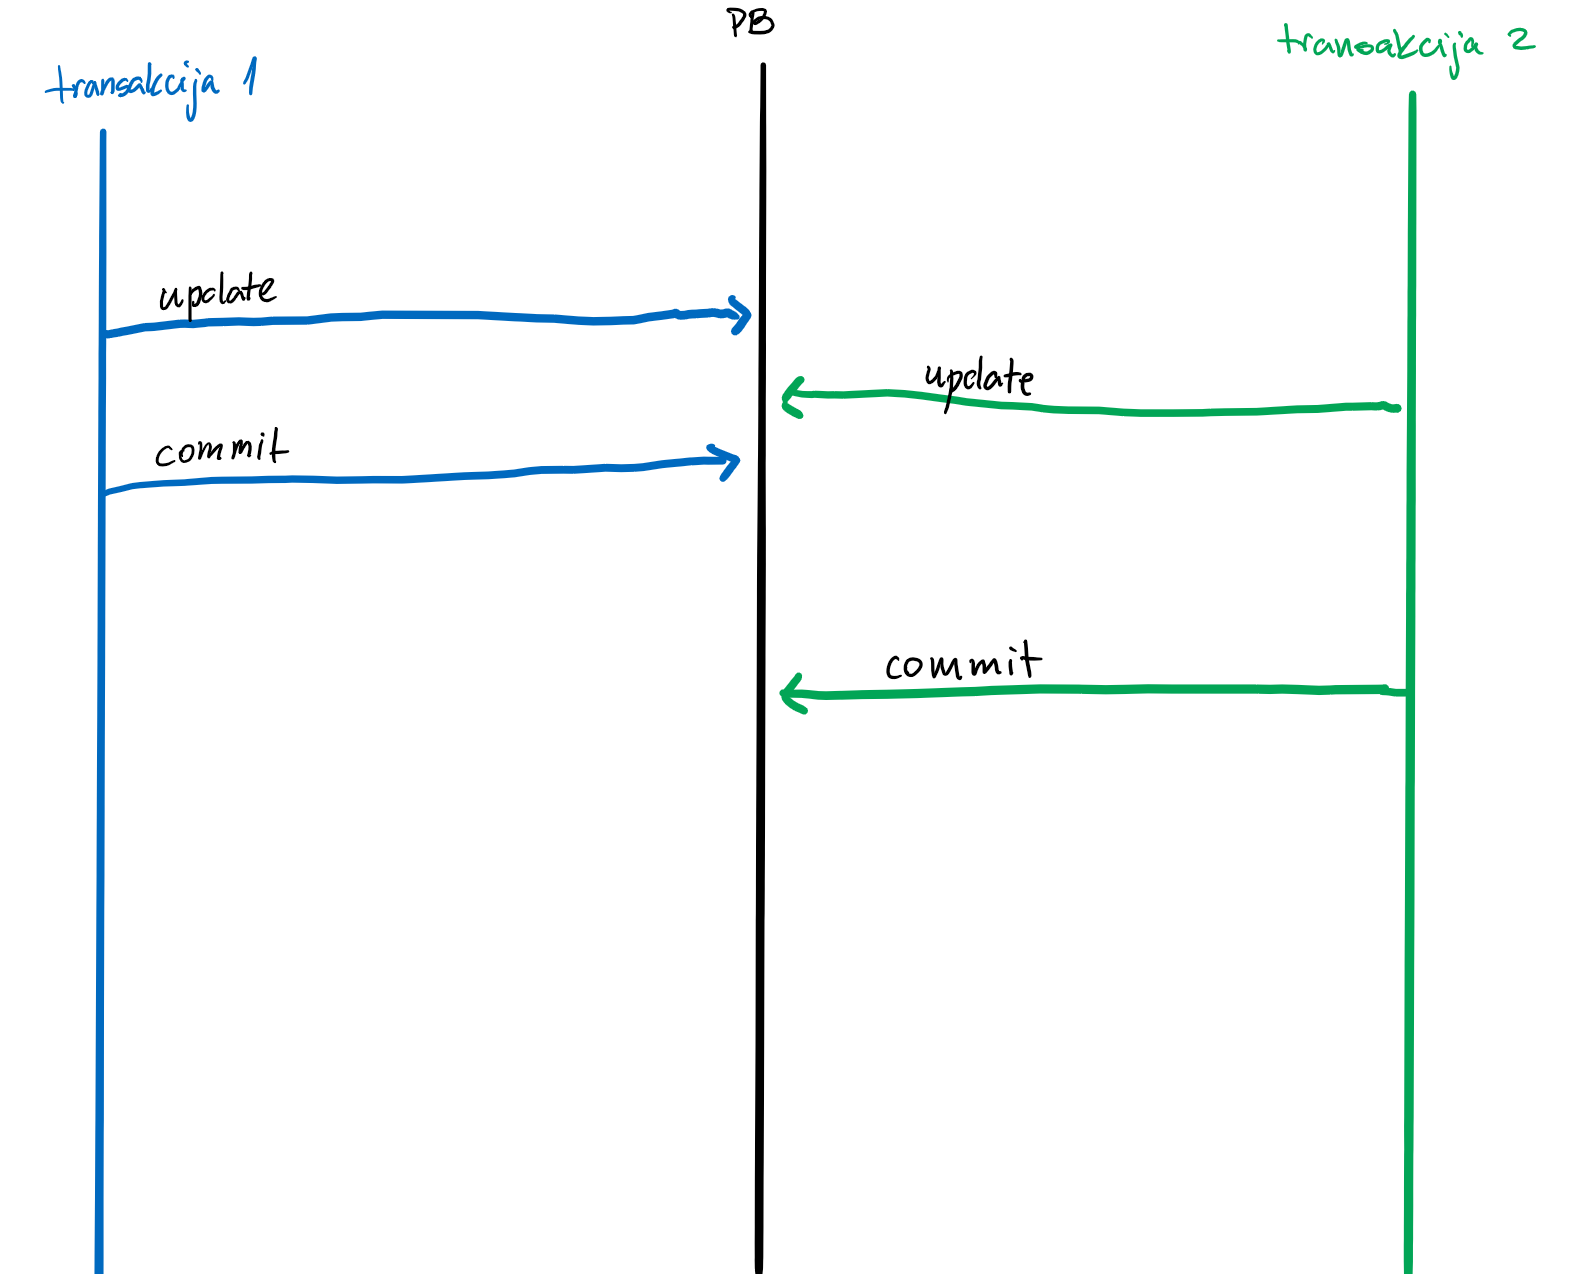
\includegraphics[width=\linewidth]{./pics/izgubljeno_azuriranje.png}

\paragraph{Rešitev}
Izgubljeno ažuriranje lahko preprečimo z uporabo stopnje izolacije \textit{REPEATABLE READ} in \textit{SERIALIZABLE}.


\end{document}